\section{Arquitectura base con el modelo C4}\label{sec:c4}

Los dos diagramas se hicieron en draw.io y sus archivos editables están en el repositorio, en \path{docs/diagramas/c4-nivel1-contexto.drawio} y \path{docs/diagramas/c4-nivel2-contenedores.drawio}.

\subsection{Diagrama de contexto (nivel 1)}

La figura~\ref{fig:c4n1} muestra a SIC-UTEQ como una sola caja, las personas que lo usan y los sistemas externos con los que habla.

Las personas son cuatro. El estudiante registra su propuesta, sube las versiones de su documento y consulta observaciones, fechas y notas. El docente actúa como director, cuando revisa el documento y registra observaciones, y como miembro del tribunal, cuando califica la sustentación. El coordinador y la comisión de titulación revisan y aprueban propuestas, asignan director y tribunal, configuran el periodo y generan actas. El administrador gestiona usuarios, roles, correo y respaldos.

Los sistemas externos son los que ya usa uteq-export: el servidor de correo institucional para los avisos, Google Drive para los archivos, servicios de IA (Gemini, Groq y un detector de texto generado) para la revisión asistida, Zoom para tutorías y sustentaciones virtuales, y un almacenamiento en la nube (Azure Blob Storage o Amazon S3) para los respaldos. El SGA de la UTEQ aparece con línea discontinua porque no hay conexión directa: el pensum, los requisitos y las deudas se exportan en Excel y se importan al sistema.

\begin{landscape}
\begin{figure}[p]
\centering
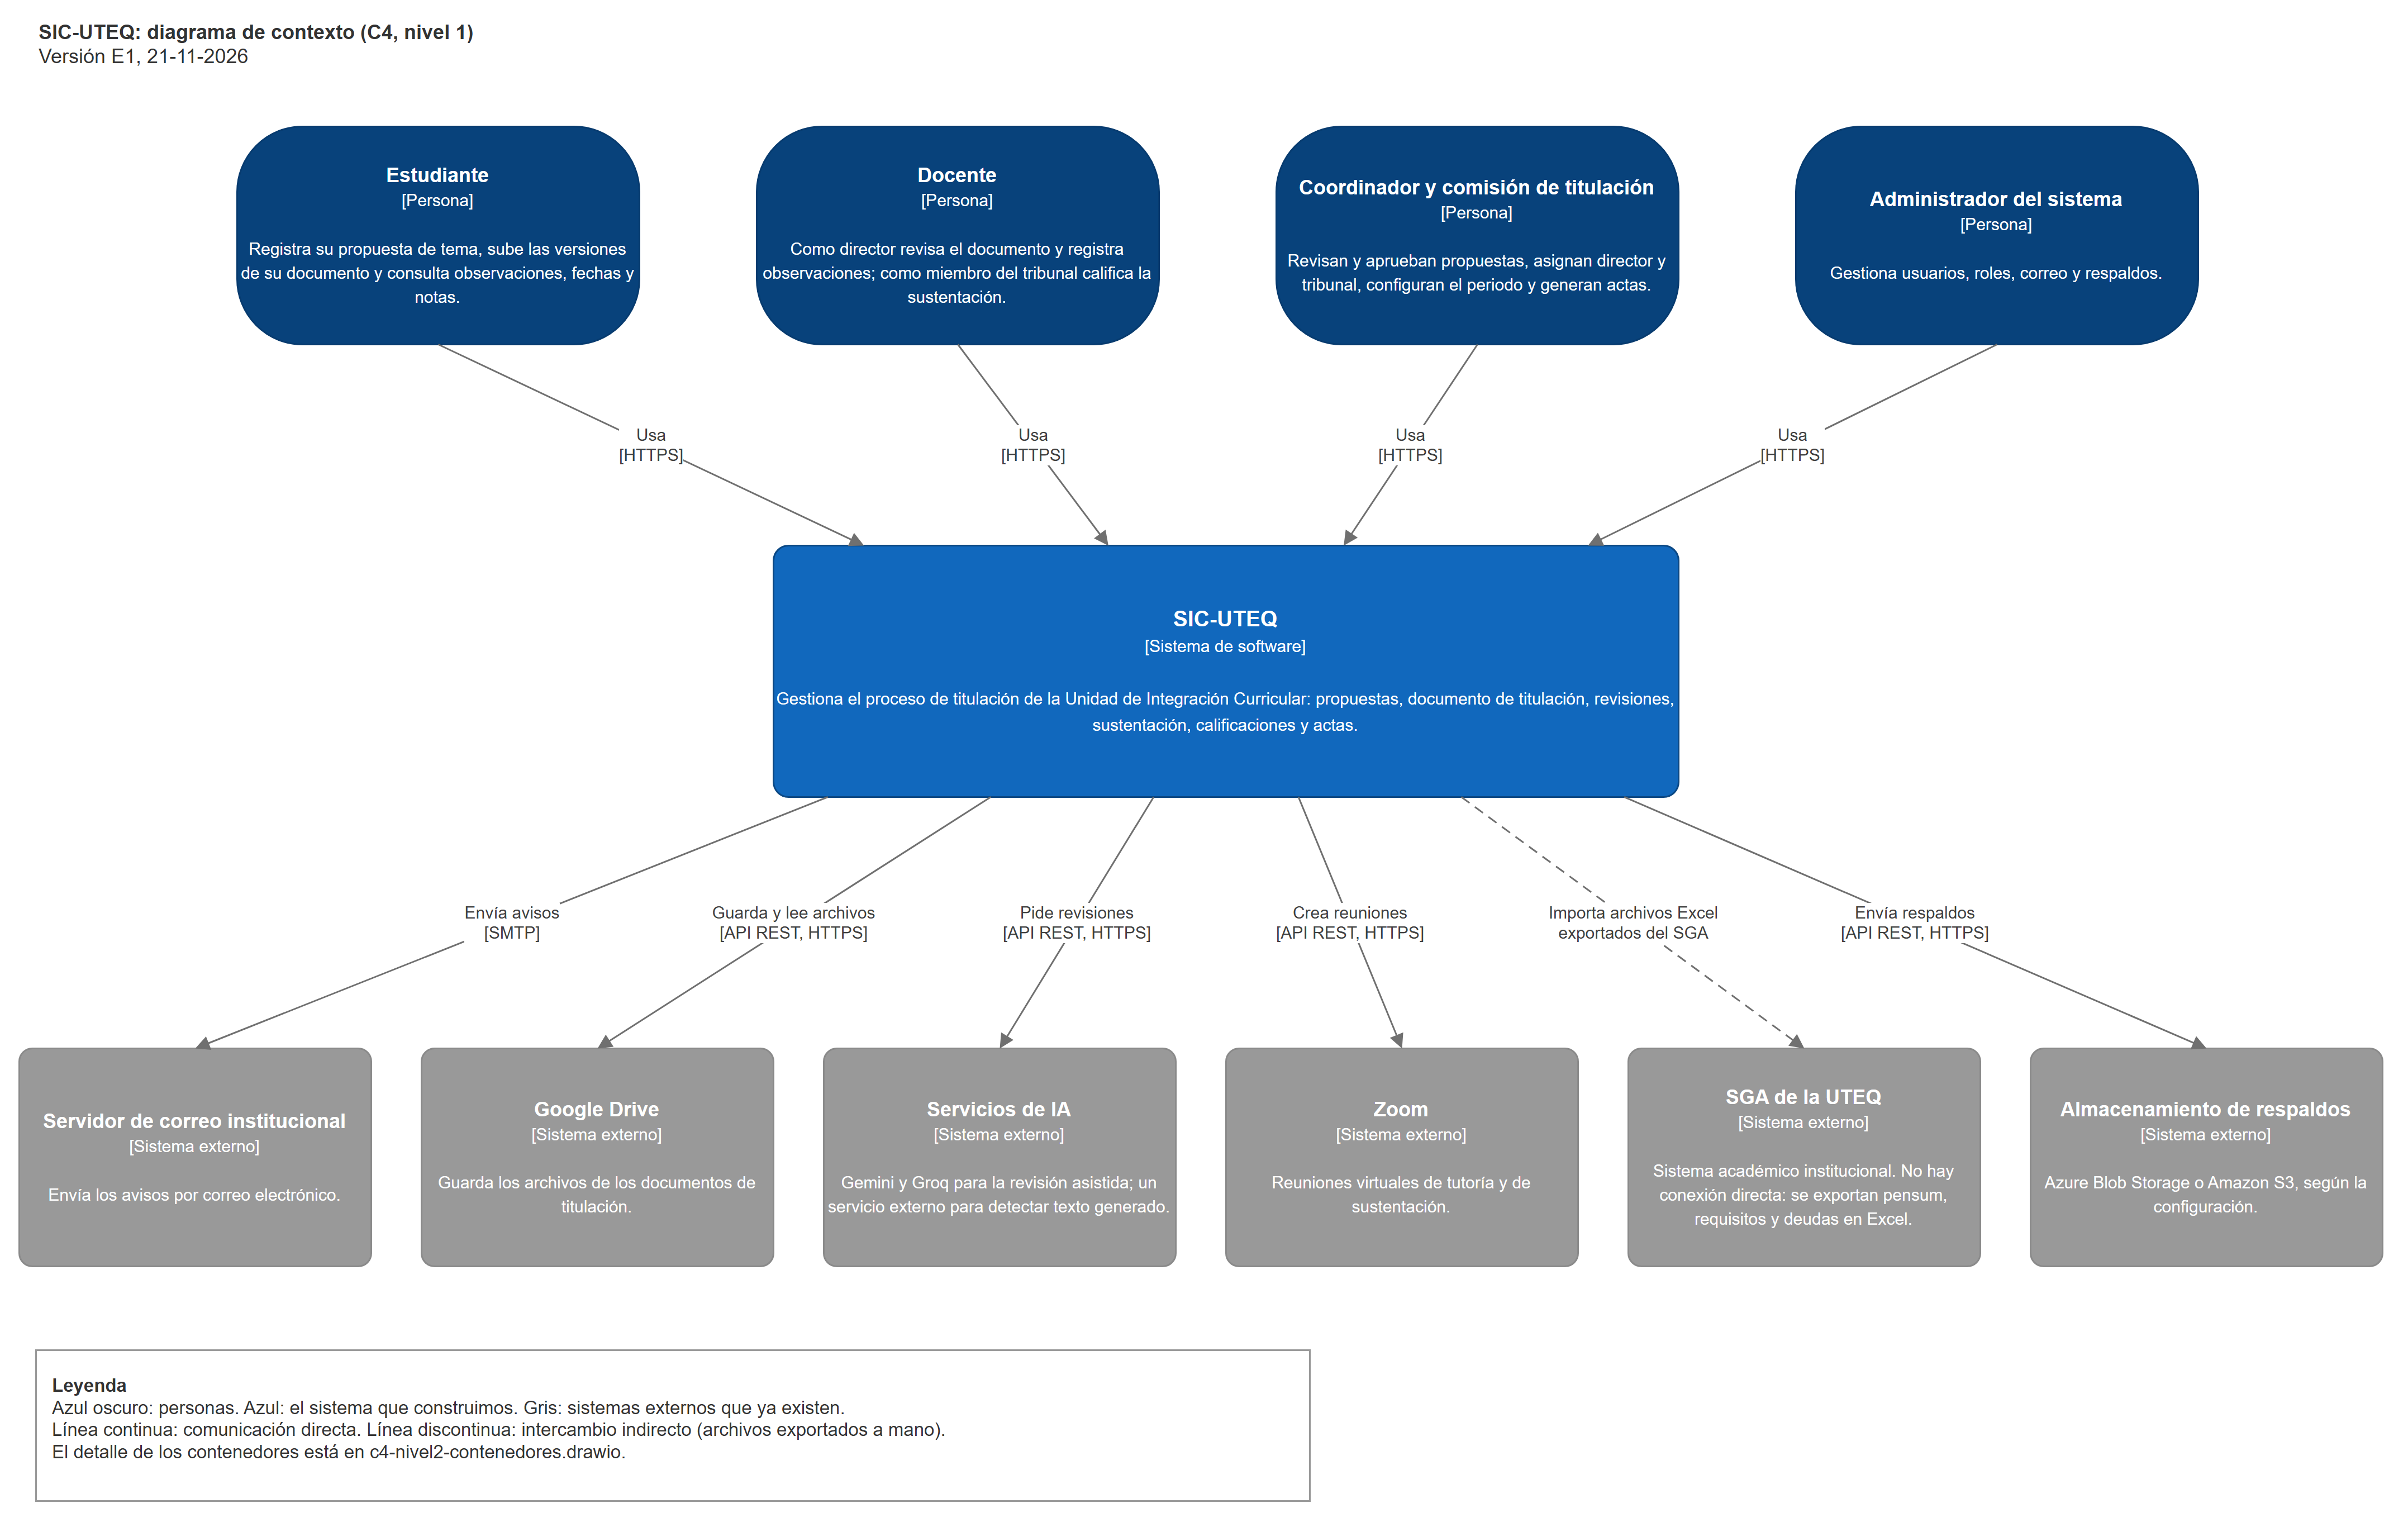
\includegraphics[width=\linewidth,height=0.9\textheight,keepaspectratio]{figuras/c4-nivel1-contexto}
\caption{Diagrama de contexto de SIC-UTEQ (C4, nivel 1)}\label{fig:c4n1}
\end{figure}
\end{landscape}

\subsection{Diagrama de contenedores (nivel 2)}

La figura~\ref{fig:c4n2} abre la caja de SIC-UTEQ. Cada flecha tiene un identificador, de I01 a I22, que corresponde a una fila de la tabla~\ref{tab:interacciones} de la sección~\ref{sec:comunicacion}.

\begin{itemize}
  \item Aplicación web en Angular 21, que corre en el navegador.
  \item API Gateway con Spring Cloud Gateway: punto de entrada único, valida el JWT y envía cada ruta a su servicio. Lo que todavía no se migra va a uteq-export.
  \item ms-usuarios y ms-propuestas (borde verde en el diagrama) ya existen en el esqueleto de E1, con datos en memoria.
  \item ms-documentos, ms-evaluacion y ms-notificaciones, el gateway y el broker RabbitMQ (borde punteado) se construyen en E2. Las bases de datos PostgreSQL de cada servicio llegan en E3.
  \item uteq-export sigue atendiendo el examen complexivo, los reportes, los respaldos y la importación del SGA mientras dure la migración.
\end{itemize}

Ningún servicio lee la base de datos de otro. Si necesita un dato ajeno, lo pide por la API o lo recibe en un evento.

\begin{landscape}
\begin{figure}[p]
\centering
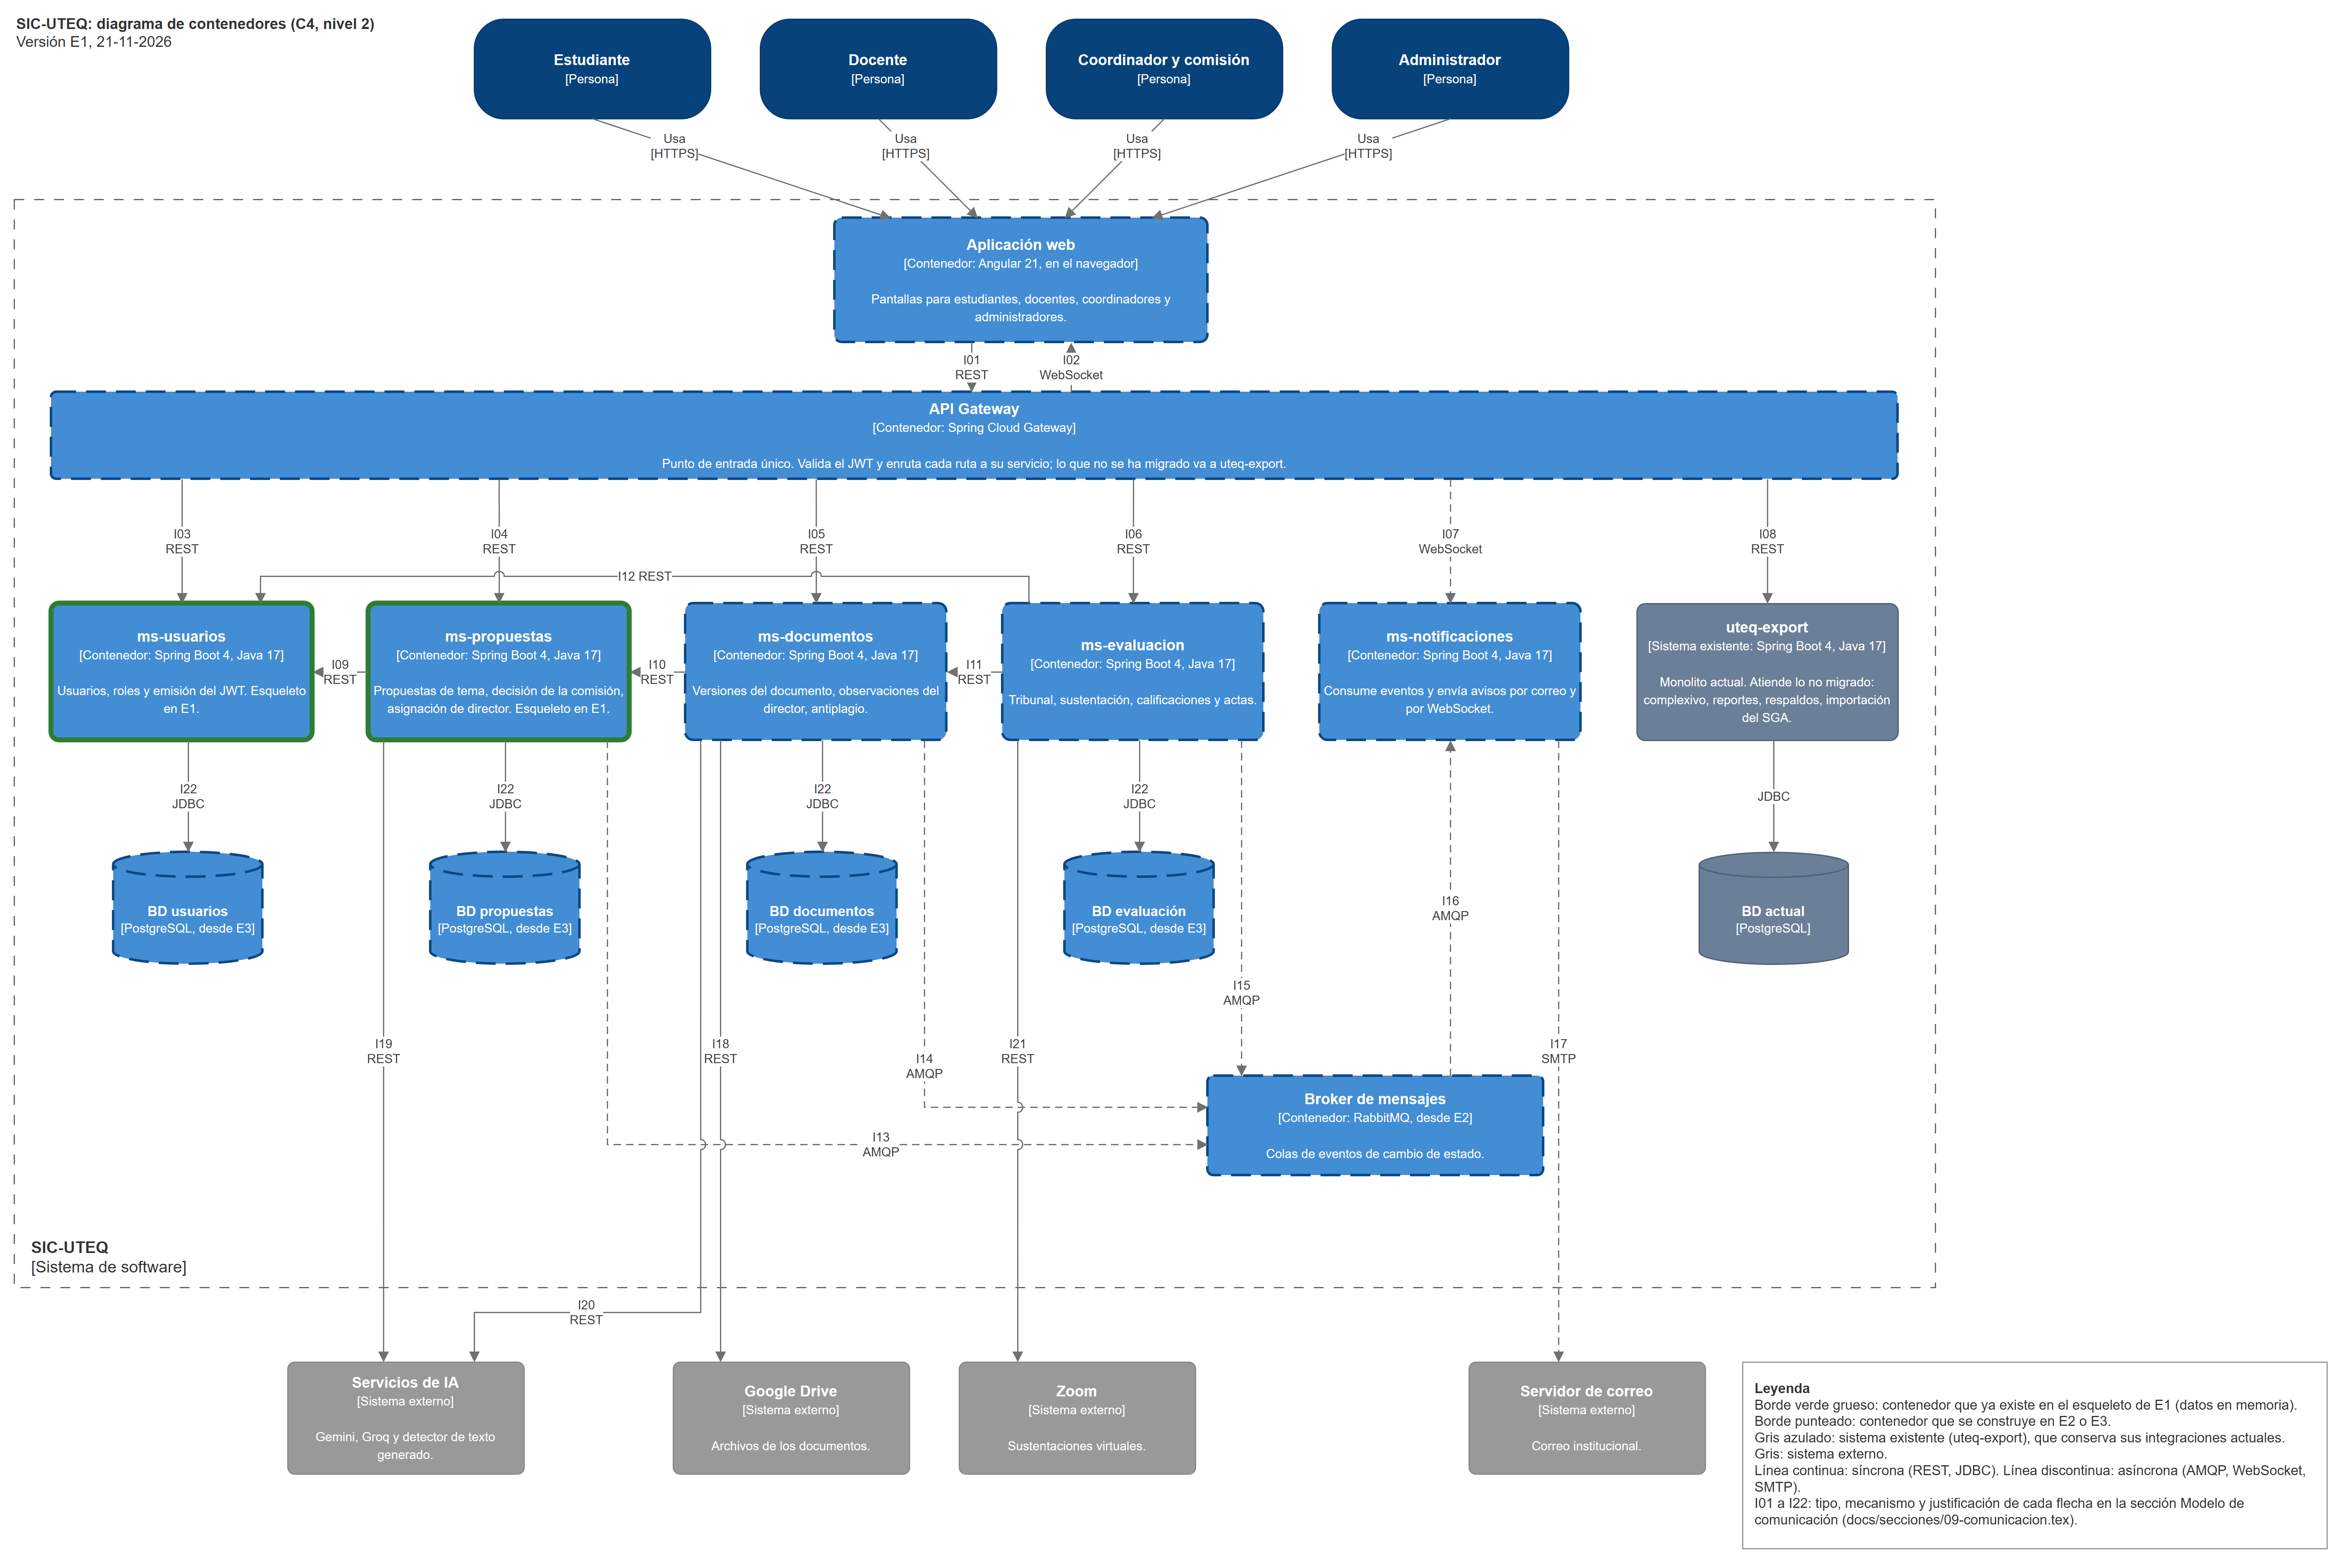
\includegraphics[width=\linewidth,height=0.9\textheight,keepaspectratio]{figuras/c4-nivel2-contenedores}
\caption{Diagrama de contenedores de SIC-UTEQ (C4, nivel 2)}\label{fig:c4n2}
\end{figure}
\end{landscape}
